% ----- auto-generated from week_03/Week*.html via pandoc -----
\chapter{Model Predictive Control --- Design and Simulation (Week 3)}
\labch{week_03}



From Receding-Horizon Optimisation to Real-Time Robotic Control

Control for Robots\\
AY 2025--26 \textbar{} 3-Hour Lecture + Activity Session

\section{Overview}

\subsection{Week 1 Recall: Computed Torque Control --- Exam Practice}

Before we begin new material, you must demonstrate command of the Week 1 content.
Take out \textbf{pen and paper}. You have \textbf{20 minutes} to answer both questions below by hand, showing every step.
These are representative of the questions you will face in the final exam.

\subsubsection{Question 1 --- Computed Torque Derivation (10 marks)}

Given a 2-DOF planar manipulator with Euler--Lagrange dynamics

\[
                        M(q)\,\ddot{q} + C(q,\dot{q})\,\dot{q} + G(q) = \tau
                    \]

derive the computed torque control law

\[
                        \tau = M(q)\bigl[\ddot{q}_d + K_D\,\dot{e} + K_P\,e\bigr] + C(q,\dot{q})\,\dot{q} + G(q)
                    \]

where \(e = q_d - q\) is the tracking error.

\textbf{Step-by-step requirements:}

\begin{enumerate}
\tightlist
\item
  Substitute the control law \(\tau\) into the equation of motion.
\item
  Cancel the Coriolis and gravity terms on both sides.
\item
  Left-multiply both sides by \(M^{-1}(q)\) and justify why \(M(q)\) must be invertible (state the positive-definiteness property).
\item
  Rearrange using \(\ddot{e} = \ddot{q}_d - \ddot{q}\) to obtain the closed-loop error dynamics:
\end{enumerate}

\[
                        \ddot{e} + K_D\,\dot{e} + K_P\,e = 0
                    \]

Explain the physical significance of this result: what kind of system does it represent, and what does it guarantee about the tracking error?

\subsubsection{Question 2 --- Lyapunov Stability Proof (10 marks)}

For the computed torque controller derived in Question 1, construct the Lyapunov candidate function:

\[
                        V(e, \dot{e}) = \frac{1}{2}\,\dot{e}^T\,M(q)\,\dot{e} \;+\; \frac{1}{2}\,e^T\,K_P\,e
                    \]

\begin{enumerate}
\tightlist
\item
  State why \(V > 0\) for all \((e, \dot{e}) \neq (0, 0)\).
\item
  Differentiate \(V\) with respect to time. Show every term in \(\dot{V}\).
\item
  Substitute the closed-loop dynamics \(M(q)\,\ddot{e} = -C(q,\dot{q})\,\dot{e} - K_D\,\dot{e} - K_P\,e\).
\item
  Apply the skew-symmetry property: \(\dot{e}^T\bigl[\dot{M}(q) - 2C(q,\dot{q})\bigr]\dot{e} = 0\).
\item
  Show that \(\dot{V} = -\dot{e}^T\,K_D\,\dot{e} \leq 0\).
\item
  Invoke LaSalle\textquotesingle s invariance principle to conclude asymptotic stability of the equilibrium \((e, \dot{e}) = (0, 0)\). State the invariance argument explicitly.
\end{enumerate}

\textbf{You have 20 minutes.} If you can reproduce both derivations cleanly, you will be able to do it in the exam. If you struggle, revise your Week 1 notes tonight. These two derivations form the foundation for everything that follows in this module.

\subsection{Learning Outcomes}

\textbf{By the end of this session, you will be able to:}

\begin{itemize}
\tightlist
\item
  \textbf{Formulate} MPC optimisation problems for robotic systems with state and control constraints
\item
  \textbf{Derive} the MPC control law from quadratic cost minimisation over a finite prediction horizon
\item
  \textbf{Implement} MPC for a 2-DOF manipulator, a differential-drive mobile robot, and a quadrotor drone
\item
  \textbf{Tune} the prediction horizon \(N\), state weight \(Q\), and control weight \(R\), and understand their effects on tracking performance, control effort, and computational cost
\item
  \textbf{Simulate} MPC controllers in MATLAB and interpret the resulting trajectory and error plots
\item
  \textbf{Compare} MPC with computed torque control in terms of model requirements, constraint handling, and computational demand
\end{itemize}

\subsection{Session Roadmap (3 Hours)}

0:00 -- 0:20

\subsubsection{Previous Week Exam Practice}

\begin{itemize}
\tightlist
\item
  Computed torque derivation --- pen and paper
\item
  Lyapunov stability proof --- pen and paper
\end{itemize}

0:20 -- 0:50

\subsubsection{MPC Theory \& Derivation}

\begin{itemize}
\tightlist
\item
  What is MPC? The predict--optimise--apply paradigm
\item
  Optimisation problem formulation
\item
  State prediction over the horizon
\item
  Quadratic cost and the optimal control law
\item
  Receding horizon strategy
\end{itemize}

0:50 -- 1:20

\subsubsection{MPC for 2-DOF Manipulator}

\begin{itemize}
\tightlist
\item
  Linearisation and discretisation of manipulator dynamics
\item
  MPC formulation with 4 states and 2 controls
\item
  Full derivation and MATLAB code
\end{itemize}

1:20 -- 1:30

\subsubsection{Break}

\begin{itemize}
\tightlist
\item
  10-minute break
\end{itemize}

1:30 -- 2:00

\subsubsection{MPC for Mobile Robot}

\begin{itemize}
\tightlist
\item
  Differential-drive kinematic model
\item
  Linearisation around reference trajectory
\item
  MPC with velocity and turning-rate constraints
\item
  Full derivation and MATLAB code
\end{itemize}

2:00 -- 2:30

\subsubsection{MPC for Quadrotor Drone}

\begin{itemize}
\tightlist
\item
  12-state quadrotor model linearised around hover
\item
  MPC with thrust and torque constraints
\item
  Full derivation and MATLAB code
\end{itemize}

2:30 -- 3:00

\subsubsection{MATLAB Implementation \& Activities}

\begin{itemize}
\tightlist
\item
  Activity 1: Horizon length tuning experiment
\item
  Activity 2: Side-by-side comparison of all three systems
\item
  Think--Pair--Share and summary
\end{itemize}

\section{MPC Theory \& Derivation}

\subsection{What Is Model Predictive Control?}

Model Predictive Control (MPC) is an optimisation-based control strategy that operates on a simple but powerful principle:
at every time step, \textbf{predict} the future behaviour of the system over a finite horizon, \textbf{optimise} a control sequence to minimise a cost function,
and \textbf{apply} only the first control action before repeating the process at the next time step.

\subsubsection{1. Predict}

Use the system model \(x_{k+1} = A\,x_k + B\,u_k\) to propagate the state forward \(N\) steps into the future, generating a predicted state trajectory \(\{x_{k+1}, x_{k+2}, \ldots, x_{k+N}\}\).

\subsubsection{2. Optimise}

Find the control sequence \(U = [u_k, u_{k+1}, \ldots, u_{k+N-1}]^T\) that minimises a cost function penalising state deviations from the reference and control effort, subject to constraints.

\subsubsection{3. Apply}

Apply only the first element \(u_k^*\) of the optimal sequence to the plant. At the next time step \(k+1\), measure the new state and repeat the entire process. This is the \textbf{receding horizon} strategy.

\emph{Figure 1: The MPC receding horizon concept. At each time step, the controller predicts future states over a finite horizon, optimises a control sequence, applies only the first input, then shifts the window forward.}

\subsection{The Optimisation Problem}

Consider a discrete-time linear time-invariant system:

\[ x_{k+1} = A\,x_k + B\,u_k \]

where \(x_k \in \mathbb{R}^n\) is the state, \(u_k \in \mathbb{R}^m\) is the control input, \(A \in \mathbb{R}^{n \times n}\) and \(B \in \mathbb{R}^{n \times m}\).

The MPC optimisation problem at time step \(k\) is:

\textbf{MPC Optimisation Problem}\\
\strut \\
\[
                    \min_{U} \; J = \sum_{i=1}^{N} \bigl(x_{k+i} - x_{\text{ref}}\bigr)^T Q \bigl(x_{k+i} - x_{\text{ref}}\bigr) \;+\; \sum_{i=0}^{N-1} u_{k+i}^T\,R\,u_{k+i}
                    \]

subject to: \(x_{k+i+1} = A\,x_{k+i} + B\,u_{k+i}\), \(\;u_{\min} \leq u_{k+i} \leq u_{\max}\), \(\;x_{\min} \leq x_{k+i} \leq x_{\max}\)

Here \(Q \succeq 0\) is the state cost matrix (penalises deviation from the reference),
\(R \succ 0\) is the control cost matrix (penalises large control inputs),
and \(N\) is the prediction horizon length.

\emph{Figure 2: MPC closed-loop control architecture. The optimizer uses a system model and constraints to compute the optimal control sequence; only the first input is applied to the plant. State feedback closes the loop.}

\subsection{State Prediction over the Horizon}

By recursively applying the dynamics, we can express all future states in terms of the current state \(x_k\) and the control sequence \(U\):

\subsubsection{Recursive State Prediction}

\textbf{Step 1:} One step ahead:

\[ x_{k+1} = A\,x_k + B\,u_k \]

\textbf{Step 2:} Two steps ahead:

\[ x_{k+2} = A\,x_{k+1} + B\,u_{k+1} = A^2\,x_k + A\,B\,u_k + B\,u_{k+1} \]

\textbf{Step 3:} General \(i\) steps ahead:

\[ x_{k+i} = A^i\,x_k + \sum_{j=0}^{i-1} A^{i-1-j}\,B\,u_{k+j} \]

\textbf{Step 4:} Stack all predictions into a single matrix equation. Define:

\[
                    \mathbf{X} = \begin{bmatrix} x_{k+1} \\ x_{k+2} \\ \vdots \\ x_{k+N} \end{bmatrix}, \quad
                    \mathbf{U} = \begin{bmatrix} u_k \\ u_{k+1} \\ \vdots \\ u_{k+N-1} \end{bmatrix}
                    \]

Then:

\[
                    \mathbf{X} = \mathcal{A}\,x_k + \mathcal{B}\,\mathbf{U}
                    \]

where:

\[
                    \mathcal{A} = \begin{bmatrix} A \\ A^2 \\ A^3 \\ \vdots \\ A^N \end{bmatrix}, \quad
                    \mathcal{B} = \begin{bmatrix}
                    B & 0 & 0 & \cdots & 0 \\
                    AB & B & 0 & \cdots & 0 \\
                    A^2B & AB & B & \cdots & 0 \\
                    \vdots & \vdots & \vdots & \ddots & \vdots \\
                    A^{N-1}B & A^{N-2}B & A^{N-3}B & \cdots & B
                    \end{bmatrix}
                    \]

\emph{Figure 3: State prediction visualization. The optimizer evaluates multiple control sequences (grey dashed) and selects the one minimizing the cost (green). Only the first control action u\_k* is applied; the rest are discarded and re-computed at the next step.}

\subsection{Quadratic Cost in Matrix Form}

Define the stacked reference \(\mathbf{X}_{\text{ref}} = [x_{\text{ref}}^T, x_{\text{ref}}^T, \ldots, x_{\text{ref}}^T]^T \in \mathbb{R}^{Nn}\)
and the block-diagonal weight matrices:

\[
                    \mathbf{Q}_N = \text{blkdiag}(Q, Q, \ldots, Q) \in \mathbb{R}^{Nn \times Nn}, \quad
                    \mathbf{R}_N = \text{blkdiag}(R, R, \ldots, R) \in \mathbb{R}^{Nm \times Nm}
                \]

Substituting \(\mathbf{X} = \mathcal{A}\,x_k + \mathcal{B}\,\mathbf{U}\) into the cost function:

\subsubsection{Cost Function Expansion}

\[
                    J = (\mathbf{X} - \mathbf{X}_{\text{ref}})^T \mathbf{Q}_N (\mathbf{X} - \mathbf{X}_{\text{ref}}) + \mathbf{U}^T \mathbf{R}_N \mathbf{U}
                    \]

Let \(\mathbf{E} = \mathbf{X}_{\text{ref}} - \mathcal{A}\,x_k\) (the "free-response error"). Then \(\mathbf{X} - \mathbf{X}_{\text{ref}} = \mathcal{B}\,\mathbf{U} - \mathbf{E}\), so:

\[
                    J = (\mathcal{B}\,\mathbf{U} - \mathbf{E})^T \mathbf{Q}_N (\mathcal{B}\,\mathbf{U} - \mathbf{E}) + \mathbf{U}^T \mathbf{R}_N \mathbf{U}
                    \]

Expanding:

\[
                    J = \mathbf{U}^T \underbrace{(\mathcal{B}^T \mathbf{Q}_N \mathcal{B} + \mathbf{R}_N)}_{H} \mathbf{U}
                    - 2\,\mathbf{E}^T \mathbf{Q}_N \mathcal{B}\,\mathbf{U}
                    + \mathbf{E}^T \mathbf{Q}_N \mathbf{E}
                    \]

This is a strictly convex quadratic in \(\mathbf{U}\) (since \(H \succ 0\) when \(R \succ 0\)), so the unique minimum is found by setting \(\frac{\partial J}{\partial \mathbf{U}} = 0\):

\[
                    2\,H\,\mathbf{U}^* - 2\,\mathcal{B}^T \mathbf{Q}_N \mathbf{E} = 0
                    \]

\subsection{The Optimal Control Law}

\textbf{MPC Optimal Control Sequence}\\
\strut \\
\[
                    \mathbf{U}^* = \bigl(\mathcal{B}^T \mathbf{Q}_N \mathcal{B} + \mathbf{R}_N\bigr)^{-1} \mathcal{B}^T \mathbf{Q}_N \bigl(\mathbf{X}_{\text{ref}} - \mathcal{A}\,x_k\bigr)
                    \]

The matrix \(H = \mathcal{B}^T \mathbf{Q}_N \mathcal{B} + \mathbf{R}_N\) is of dimension \(Nm \times Nm\). It must be inverted (or factorised) at every time step. This is the primary computational cost of MPC.

\subsection{Receding Horizon: Apply Only the First Input}

The full optimal sequence is \(\mathbf{U}^* = [u_k^{*T}, u_{k+1}^{*T}, \ldots, u_{k+N-1}^{*T}]^T\).
In the receding-horizon strategy, we \textbf{apply only the first element}:

\[ u_k = u_k^* = \text{first } m \text{ entries of } \mathbf{U}^* \]

At the next time step, the state \(x_{k+1}\) is measured (or estimated), and the entire optimisation is re-solved.
This feedback mechanism gives MPC its robustness to disturbances and model errors.

\emph{Figure 4: MPC flowchart showing the predict-optimise-apply loop. The key insight is that only the first control input is applied (highlighted in green), and the entire optimisation is re-solved at every time step.}

\subsubsection{Think--Pair--Share (3 min)}

\textbf{Question:} Why does MPC re-solve the optimisation at every time step instead of applying the entire precomputed sequence \(\mathbf{U}^*\)?

Hint: Think about what happens if the model is imperfect, or if a disturbance pushes the state away from the predicted trajectory.
Compare with open-loop vs closed-loop control.

\begin{verbatim}
                    PSEUDOCODE — MPC Receding Horizon Algorithm
\end{verbatim}

INITIALISE: state x\_0, horizon N, weights Q and R
BUILD: prediction matrices A\_cal and B\_cal from (A, B, N)
BUILD: block-diagonal weights Q\_N = blkdiag(Q,...,Q), R\_N = blkdiag(R,...,R)
COMPUTE: H = B\_cal\textquotesingle{} * Q\_N * B\_cal + R\_N
COMPUTE: H\_inv = inv(H) (do this ONCE if A, B are constant)
FOR k = 0, 1, 2, ... DO
MEASURE (or estimate) current state x\_k
BUILD reference vector: X\_ref = {[}x\_ref; x\_ref; ...; x\_ref{]} (N copies)
COMPUTE free-response error: E = X\_ref - A\_cal * x\_k
COMPUTE optimal sequence: U\_star = H\_inv * B\_cal\textquotesingle{} * Q\_N * E
EXTRACT first control: u\_k = U\_star(1:m)
APPLY u\_k to the plant
ADVANCE to next time step
END FOR

\subsection{Effect of Tuning Parameters}

\begingroup\footnotesize
\begin{longtable}[]{@{}lll@{}}
\toprule\noalign{}
Parameter & Increase Effect & Decrease Effect \\
\midrule\noalign{}
\endhead
\bottomrule\noalign{}
\endlastfoot
Prediction horizon \(N\) & Better anticipation of future references; more stable; higher computational cost (\(O(N^3 m^3)\)) & More myopic; may oscillate or become unstable; cheaper to compute \\
State weight \(Q\) & Tighter tracking; more aggressive control; risk of actuator saturation & Relaxed tracking; smoother control inputs; larger steady-state error \\
Control weight \(R\) & Penalises large inputs; smoother control; slower response; energy-efficient & Allows large inputs; fast response; risk of actuator damage \\
\end{longtable}\endgroup

\textbf{Practical Guideline:} Start with \(Q = I\), \(R = 0.1 I\), and \(N = 10\). Then adjust: increase \(Q\) if tracking is too loose, increase \(R\) if control inputs saturate, and increase \(N\) until performance no longer improves significantly.

\section{MPC for 2-DOF Manipulator}

\subsection{The Nonlinear Dynamics}

Recall from Week 1 the 2-DOF planar manipulator dynamics:

\[
                    M(q)\,\ddot{q} + C(q,\dot{q})\,\dot{q} + G(q) = \tau
                \]

with state vector \(x = [q_1, q_2, \dot{q}_1, \dot{q}_2]^T \in \mathbb{R}^4\) and control input \(u = [\tau_1, \tau_2]^T \in \mathbb{R}^2\).

\emph{Figure 5: 2-DOF planar manipulator with joint angles θ1, θ2, link lengths l1, l2, masses m1, m2, and torque inputs τ1, τ2. The coordinate frame is shown at the base with gravity acting downward.}

\subsection{Linearisation around an Operating Point}

MPC (in its basic linear form) requires a linear discrete-time model. We linearise the manipulator dynamics around a nominal operating point
\((q_0, \dot{q}_0) = (0, 0)\) (the hanging-down equilibrium).

\subsubsection{Linearisation Procedure}

The continuous-time state-space form is:

\[
                    \dot{x} = f(x, u) = \begin{bmatrix} \dot{q} \\ M^{-1}(q)\bigl[\tau - C(q,\dot{q})\dot{q} - G(q)\bigr] \end{bmatrix}
                    \]

At the operating point \(x_0 = [0, 0, 0, 0]^T\), \(u_0 = G(q_0)\) (the torque needed to hold the arm at \(q_0\)):

\[
                    A_c = \left.\frac{\partial f}{\partial x}\right|_{x_0, u_0}, \quad
                    B_c = \left.\frac{\partial f}{\partial u}\right|_{x_0, u_0}
                    \]

For the 2-DOF arm with \(m_1 = m_2 = 1\,\text{kg}\), \(l_1 = l_2 = 1\,\text{m}\), evaluated at \(q = 0\):

\[
                    M(0) = \begin{bmatrix} m_1 l_1^2 + m_2(l_1^2 + l_2^2 + 2l_1 l_2) & m_2(l_2^2 + l_1 l_2) \\ m_2(l_2^2 + l_1 l_2) & m_2 l_2^2 \end{bmatrix}
                    = \begin{bmatrix} 4 & 2 \\ 2 & 1 \end{bmatrix}
                    \]

Since \(C(q, 0) = 0\) at zero velocity, and the gravity linearisation yields stiffness terms, the linearised continuous-time system is:

\[
                    A_c = \begin{bmatrix}
                    0 & 0 & 1 & 0 \\
                    0 & 0 & 0 & 1 \\
                    0 & 0 & 0 & 0 \\
                    0 & 0 & 0 & 0
                    \end{bmatrix}, \quad
                    B_c = \begin{bmatrix}
                    0_{2 \times 2} \\
                    M^{-1}(q_0)
                    \end{bmatrix}
                    \]

Computing \(M^{-1}(0)\): since \(\det(M(0)) = 4 \cdot 1 - 2 \cdot 2 = 0\)... Note that \(M(0)\) is singular at this particular configuration because we used point masses at link tips. In practice we use the more general parametrisation with \(l_{c1}, l_{c2}\). For our MATLAB implementation, we evaluate at a slightly offset configuration \(q_0 = [0.1, 0.1]^T\) to ensure non-singularity, giving:

\[
                    M(q_0) \approx \begin{bmatrix} 3.96 & 1.99 \\ 1.99 & 1.0 \end{bmatrix}, \quad
                    M^{-1}(q_0) \approx \begin{bmatrix} 50.25 & -100.0 \\ -100.0 & 199.0 \end{bmatrix}
                    \]

\subsection{Discretisation}

Using the zero-order hold (ZOH) method with sampling time \(\Delta t\):

\[
                    A_d = e^{A_c \Delta t} \approx I + A_c \Delta t, \quad
                    B_d \approx B_c \Delta t
                    \]

First-order Euler approximation, valid for small \(\Delta t\).

\subsection{MPC Design for the Manipulator}

State: \(x = [q_1, q_2, \dot{q}_1, \dot{q}_2]^T\), Control: \(u = [\tau_1, \tau_2]^T\)

\subsubsection{Weight Matrix Selection}

We want tight tracking of joint positions but allow velocities to deviate more freely:

\[
                    Q = \text{diag}(100, 100, 1, 1), \quad R = \text{diag}(0.01, 0.01)
                    \]

The ratio \(Q/R\) determines aggressiveness: here \(q_{ii}/r_{ii} = 10{,}000\), so the controller strongly prioritises position tracking over control effort economy.

With prediction horizon \(N = 20\) and \(\Delta t = 0.01\,\text{s}\), we build the prediction matrices \(\mathcal{A} \in \mathbb{R}^{80 \times 4}\) and \(\mathcal{B} \in \mathbb{R}^{80 \times 40}\),
then compute the Hessian \(H = \mathcal{B}^T \mathbf{Q}_N \mathcal{B} + \mathbf{R}_N \in \mathbb{R}^{40 \times 40}\).

\subsection{MATLAB Implementation --- Manipulator MPC}

\begin{verbatim}
%% === MPC for 2-DOF Manipulator ===
% System parameters
params.m1 = 1; params.m2 = 1;
params.l1 = 1; params.l2 = 1;
params.g = 9.81;

% Linearisation point
q0 = [0.1; 0.1]; dq0 = [0; 0];

% Build M(q0), compute M_inv
c2 = cos(q0(2));
M11 = params.m1*params.l1^2 + params.m2*(params.l1^2 + params.l2^2 + 2*params.l1*params.l2*c2);
M12 = params.m2*(params.l2^2 + params.l1*params.l2*c2);
M22 = params.m2*params.l2^2;
M0 = [M11, M12; M12, M22];
M0_inv = inv(M0);

% Continuous-time A, B (linearised around q0, dq0=0)
Ac = [zeros(2), eye(2); zeros(2), zeros(2)];
Bc = [zeros(2); M0_inv];

% Discretise (Euler, dt = 0.01 s)
dt = 0.01;
Ad = eye(4) + Ac*dt;
Bd = Bc*dt;

% MPC parameters
N = 20;                          % Prediction horizon
Q = diag([100, 100, 1, 1]);     % State weight
R = diag([0.01, 0.01]);         % Control weight

% Build prediction matrices
n = 4; m = 2;
A_cal = zeros(n*N, n);
B_cal = zeros(n*N, m*N);
for i = 1:N
    A_cal((i-1)*n+1:i*n, :) = Ad^i;
    for j = 1:i
        B_cal((i-1)*n+1:i*n, (j-1)*m+1:j*m) = Ad^(i-j) * Bd;
    end
end

% Block-diagonal weights
Q_N = kron(eye(N), Q);
R_N = kron(eye(N), R);

% Hessian and its inverse (constant for LTI system)
H = B_cal' * Q_N * B_cal + R_N;
H_inv = inv(H);
F = B_cal' * Q_N;

% Simulation
t_span = 0:dt:20;
x = [0; 0; 0; 0];  % Initial state
x_hist = zeros(4, length(t_span));
u_hist = zeros(2, length(t_span));
x_hist(:,1) = x;

for k = 1:length(t_span)-1
    t = t_span(k);

    % Reference trajectory (sinusoidal)
    x_ref_k = zeros(n*N, 1);
    for i = 1:N
        t_future = t + i*dt;
        x_ref_k((i-1)*n+1:i*n) = [0.5*sin(t_future); 0.5*cos(t_future); ...
                                    0.5*cos(t_future); -0.5*sin(t_future)];
    end

    % MPC optimal control
    E = x_ref_k - A_cal * x;
    U_star = H_inv * F * E;
    u = U_star(1:m);  % Apply first control only

    % Clamp torques (constraint enforcement)
    u = max(min(u, 50), -50);

    % Simulate true nonlinear dynamics (one Euler step)
    q = x(1:2); dq = x(3:4);
    [M_true, C_true, G_true] = manipulator_model(q, dq, params);
    ddq = M_true \ (u - C_true*dq - G_true);
    x = x + [dq; ddq]*dt;

    x_hist(:,k+1) = x;
    u_hist(:,k) = u;
end
\end{verbatim}

\textbf{Note:} The controller uses a \emph{linear} model, but the plant simulation uses the \emph{full nonlinear} dynamics. This mismatch is realistic and tests the robustness of MPC.

\section{MPC for Differential-Drive Mobile Robot}

\subsection{Kinematic Model}

A differential-drive mobile robot (e.g., TurtleBot) moves in the plane with state \(x = [p_x, p_y, \theta]^T\) (position and heading) and control inputs \(u = [v, \omega]^T\) (linear and angular velocity):

\textbf{Nonlinear Kinematic Model}\\
\strut \\
\[
                    \begin{bmatrix} \dot{p}_x \\ \dot{p}_y \\ \dot{\theta} \end{bmatrix}
                    = \begin{bmatrix} v\,\cos\theta \\ v\,\sin\theta \\ \omega \end{bmatrix}
                    \]

\emph{Figure 6: Top-down view of a differential-drive mobile robot. The robot state is (p\_x, p\_y, θ), controlled by linear velocity v and angular velocity ω. The reference path is shown as a dashed curve.}

Discretised with Euler integration at sampling time \(\Delta t\):

\[
                \begin{aligned}
                p_{x,k+1} &= p_{x,k} + v_k \cos(\theta_k)\,\Delta t \\
                p_{y,k+1} &= p_{y,k} + v_k \sin(\theta_k)\,\Delta t \\
                \theta_{k+1} &= \theta_k + \omega_k\,\Delta t
                \end{aligned}
                \]

\subsection{Linearisation around a Reference Trajectory}

\subsubsection{Jacobian Linearisation}

Let the reference trajectory be \((p_x^r(t), p_y^r(t), \theta^r(t))\) with reference controls \((v^r(t), \omega^r(t))\).
Define error variables:

\[
                    \delta x = x - x^r, \quad \delta u = u - u^r
                    \]

The Jacobians of the continuous-time model at the reference are:

\[
                    A_c = \frac{\partial f}{\partial x}\bigg|_{x^r, u^r} = \begin{bmatrix}
                    0 & 0 & -v^r \sin\theta^r \\
                    0 & 0 & v^r \cos\theta^r \\
                    0 & 0 & 0
                    \end{bmatrix}
                    \]
\[
                    B_c = \frac{\partial f}{\partial u}\bigg|_{x^r, u^r} = \begin{bmatrix}
                    \cos\theta^r & 0 \\
                    \sin\theta^r & 0 \\
                    0 & 1
                    \end{bmatrix}
                    \]

For simplicity, we linearise around \(\theta^r = 0\) (heading east) and \(v^r = 2.5\,\text{m/s}\):

\[
                    A_c = \begin{bmatrix} 0 & 0 & 0 \\ 0 & 0 & 2.5 \\ 0 & 0 & 0 \end{bmatrix}, \quad
                    B_c = \begin{bmatrix} 1 & 0 \\ 0 & 0 \\ 0 & 1 \end{bmatrix}
                    \]

Discretised:

\[
                    A_d = I + A_c \Delta t, \quad B_d = B_c \Delta t
                    \]

\subsection{Constraints}

\begingroup\footnotesize
\begin{longtable}[]{@{}lll@{}}
\toprule\noalign{}
Constraint & Physical Meaning & Value \\
\midrule\noalign{}
\endhead
\bottomrule\noalign{}
\endlastfoot
\(0 \leq v \leq 5\,\text{m/s}\) & The robot cannot move backwards (for safety) and has a maximum speed & {[}0, 5{]} \\
\(-2 \leq \omega \leq 2\,\text{rad/s}\) & Maximum turning rate limited by wheel motors & {[}-2, 2{]} \\
\end{longtable}\endgroup

\subsection{MPC Design}

State: \(x = [p_x, p_y, \theta]^T\), Control: \(u = [v, \omega]^T\), Horizon: \(N = 15\), Weights:

\[ Q = \text{diag}(50, 50, 10), \quad R = \text{diag}(0.1, 0.1) \]

The higher weight on position relative to heading ensures the robot prioritises reaching the correct \((x, y)\) location, with heading as a secondary objective.

\subsection{MATLAB Implementation --- Mobile Robot MPC}

\begin{verbatim}
%% === MPC for Differential-Drive Mobile Robot ===
% Linearisation parameters
v_ref = 2.5;  % Reference linear velocity
dt = 0.05;    % Sampling time

% Linearised system (around theta = 0, v = v_ref)
Ac_mob = [0, 0, 0; 0, 0, v_ref; 0, 0, 0];
Bc_mob = [1, 0; 0, 0; 0, 1];

Ad_mob = eye(3) + Ac_mob*dt;
Bd_mob = Bc_mob*dt;

% MPC parameters
N_mob = 15;
Q_mob = diag([50, 50, 10]);
R_mob = diag([0.1, 0.1]);
n_mob = 3; m_mob = 2;

% Build prediction matrices
A_cal_mob = zeros(n_mob*N_mob, n_mob);
B_cal_mob = zeros(n_mob*N_mob, m_mob*N_mob);
for i = 1:N_mob
    A_cal_mob((i-1)*n_mob+1:i*n_mob, :) = Ad_mob^i;
    for j = 1:i
        B_cal_mob((i-1)*n_mob+1:i*n_mob, (j-1)*m_mob+1:j*m_mob) = Ad_mob^(i-j)*Bd_mob;
    end
end

Q_N_mob = kron(eye(N_mob), Q_mob);
R_N_mob = kron(eye(N_mob), R_mob);
H_mob = B_cal_mob' * Q_N_mob * B_cal_mob + R_N_mob;
H_inv_mob = inv(H_mob);
F_mob = B_cal_mob' * Q_N_mob;

% Simulation
t_span_mob = 0:dt:20;
x_mob = [0; 0; 0];
x_hist_mob = zeros(3, length(t_span_mob));
u_hist_mob = zeros(2, length(t_span_mob));
x_hist_mob(:,1) = x_mob;

% Circular reference trajectory (radius = 5 m)
R_circle = 5; omega_circle = 0.5;

for k = 1:length(t_span_mob)-1
    t = t_span_mob(k);

    % Build reference over horizon
    x_ref_mob = zeros(n_mob*N_mob, 1);
    for i = 1:N_mob
        t_f = t + i*dt;
        x_ref_mob((i-1)*n_mob+1:i*n_mob) = [R_circle*cos(omega_circle*t_f); ...
                                               R_circle*sin(omega_circle*t_f); ...
                                               omega_circle*t_f + pi/2];
    end

    % MPC solve
    E_mob = x_ref_mob - A_cal_mob * x_mob;
    U_star_mob = H_inv_mob * F_mob * E_mob;
    u_mob = U_star_mob(1:m_mob);

    % Enforce constraints
    u_mob(1) = max(min(u_mob(1), 5), 0);     % v in [0, 5]
    u_mob(2) = max(min(u_mob(2), 2), -2);    % omega in [-2, 2]

    % True nonlinear dynamics (Euler integration)
    theta = x_mob(3);
    x_mob = x_mob + [u_mob(1)*cos(theta); u_mob(1)*sin(theta); u_mob(2)]*dt;

    x_hist_mob(:,k+1) = x_mob;
    u_hist_mob(:,k) = u_mob;
end
\end{verbatim}

\textbf{Linearisation Caveat:} The linearisation is performed at a single operating point. When the robot heading \(\theta\) deviates significantly from \(\theta^r = 0\), the linear model becomes inaccurate. In practice, one re-linearises at each time step (forming a time-varying linear MPC), or uses nonlinear MPC.

\section{MPC for Quadrotor Drone}

\subsection{The 12-State Quadrotor Model}

A quadrotor has 6 degrees of freedom (3 translational + 3 rotational), leading to a 12-dimensional state vector:

\[
                    x = \begin{bmatrix} p_x \\ p_y \\ p_z \\ v_x \\ v_y \\ v_z \\ \phi \\ \theta \\ \psi \\ \omega_x \\ \omega_y \\ \omega_z \end{bmatrix}
                    \quad \text{(position, velocity, Euler angles, angular rates)}
                    \]

\emph{Figure 7: Quadrotor UAV schematic showing four rotors with alternating CW/CCW rotation directions, thrust forces F1-F4, body frame axes (x\_B, y\_B, z\_B), and Euler angles (roll φ, pitch θ, yaw ψ). The total thrust is T = F1+F2+F3+F4.}

The control inputs are thrust and three body-frame torques:

\[
                u = \begin{bmatrix} T \\ \tau_x \\ \tau_y \\ \tau_z \end{bmatrix}
                \]

\subsection{Nonlinear Equations of Motion}

\subsubsection{Full Quadrotor Dynamics}

\textbf{Translational dynamics} (Newton\textquotesingle s second law in the world frame):

\[
                    \begin{aligned}
                    \dot{v}_x &= \frac{T}{m}\bigl(\cos\phi\sin\theta\cos\psi + \sin\phi\sin\psi\bigr) \\
                    \dot{v}_y &= \frac{T}{m}\bigl(\cos\phi\sin\theta\sin\psi - \sin\phi\cos\psi\bigr) \\
                    \dot{v}_z &= \frac{T}{m}\cos\phi\cos\theta - g
                    \end{aligned}
                    \]

\textbf{Rotational dynamics} (Euler\textquotesingle s equations for a symmetric body):

\[
                    \begin{aligned}
                    \dot{\omega}_x &= \frac{\tau_x}{I_{xx}} + \frac{(I_{yy} - I_{zz})}{I_{xx}}\omega_y\omega_z \\
                    \dot{\omega}_y &= \frac{\tau_y}{I_{yy}} + \frac{(I_{zz} - I_{xx})}{I_{yy}}\omega_x\omega_z \\
                    \dot{\omega}_z &= \frac{\tau_z}{I_{zz}} + \frac{(I_{xx} - I_{yy})}{I_{zz}}\omega_x\omega_y
                    \end{aligned}
                    \]

\subsection{Linearisation around Hover}

At hover, all velocities and angular rates are zero, \(\phi = \theta = \psi = 0\), and the thrust equals gravity: \(T_0 = mg\).
The linearised continuous-time system simplifies considerably because the trigonometric functions reduce to their small-angle approximations and the cross-coupling terms in Euler\textquotesingle s equations vanish:

\subsubsection{Linearised Hover Dynamics}

At hover (\(\phi = \theta = \psi = 0\), \(T_0 = mg\)):

\[
                    \dot{v}_x \approx g\,\theta, \quad
                    \dot{v}_y \approx -g\,\phi, \quad
                    \dot{v}_z \approx \frac{T - mg}{m}
                    \]
\[
                    \dot{\omega}_x \approx \frac{\tau_x}{I_{xx}}, \quad
                    \dot{\omega}_y \approx \frac{\tau_y}{I_{yy}}, \quad
                    \dot{\omega}_z \approx \frac{\tau_z}{I_{zz}}
                    \]

The linearised state-space matrices become:

\[
                    A_c = \begin{bmatrix}
                    0_3 & I_3 & 0_3 & 0_3 \\
                    0_3 & 0_3 & G_{\text{lin}} & 0_3 \\
                    0_3 & 0_3 & 0_3 & I_3 \\
                    0_3 & 0_3 & 0_3 & 0_3
                    \end{bmatrix}, \quad
                    B_c = \begin{bmatrix}
                    0_3 \\ B_T \\ 0_3 \\ B_\tau
                    \end{bmatrix}
                    \]

where the coupling matrix \(G_{\text{lin}}\) and input matrices are:

\[
                    G_{\text{lin}} = \begin{bmatrix} 0 & g & 0 \\ -g & 0 & 0 \\ 0 & 0 & 0 \end{bmatrix}, \quad
                    B_T = \begin{bmatrix} 0 \\ 0 \\ 1/m \end{bmatrix} \begin{bmatrix} 1 & 0 & 0 & 0 \end{bmatrix}, \quad
                    B_\tau = \text{diag}\!\left(\frac{1}{I_{xx}}, \frac{1}{I_{yy}}, \frac{1}{I_{zz}}\right) \begin{bmatrix} 0 & I_3 \end{bmatrix}
                    \]

\subsection{MPC Design for the Quadrotor}

State dimension: \(n = 12\), Control dimension: \(m = 4\), Horizon: \(N = 15\).

\[
                    Q = \text{diag}(\underbrace{80, 80, 120}_{\text{position}}, \underbrace{1, 1, 1}_{\text{velocity}}, \underbrace{50, 50, 50}_{\text{orientation}}, \underbrace{1, 1, 1}_{\text{angular rate}})
                    \]
\[
                    R = \text{diag}(0.1, 0.1, 0.1, 0.1)
                    \]

\subsection{Constraints}

\begingroup\footnotesize
\begin{longtable}[]{@{}lll@{}}
\toprule\noalign{}
Constraint & Physical Meaning & Value \\
\midrule\noalign{}
\endhead
\bottomrule\noalign{}
\endlastfoot
\(0 \leq T \leq 2mg\) & Thrust cannot be negative; max is twice the hover thrust & {[}0, 19.62{]} N \\
\(-2 \leq \tau_x, \tau_y, \tau_z \leq 2\) & Maximum body torques from motor differentials & {[}-2, 2{]} N·m \\
\(-30^\circ \leq \phi, \theta \leq 30^\circ\) & Tilt angle limits for safety & {[}-0.524, 0.524{]} rad \\
\end{longtable}\endgroup

\subsection{MATLAB Implementation --- Quadrotor MPC}

\begin{verbatim}
%% === MPC for Quadrotor Drone ===
% Physical parameters
quad.m = 1.0;
quad.Ixx = 0.1; quad.Iyy = 0.1; quad.Izz = 0.2;
quad.g = 9.81;

dt_q = 0.02;  % Sampling time (50 Hz)
n_q = 12; m_q = 4;

% Linearised continuous-time matrices (hover)
Ac_q = zeros(12,12);
Ac_q(1:3, 4:6) = eye(3);                 % dp/dt = v
Ac_q(4,8) = quad.g;                      % dvx/dt = g*theta
Ac_q(5,7) = -quad.g;                     % dvy/dt = -g*phi
Ac_q(7:9, 10:12) = eye(3);               % datt/dt = omega

Bc_q = zeros(12,4);
Bc_q(6,1) = 1/quad.m;                    % dvz/dt = T/m
Bc_q(10,2) = 1/quad.Ixx;                 % domega_x/dt = tau_x/Ixx
Bc_q(11,3) = 1/quad.Iyy;                 % domega_y/dt = tau_y/Iyy
Bc_q(12,4) = 1/quad.Izz;                 % domega_z/dt = tau_z/Izz

% Discretise
Ad_q = eye(12) + Ac_q*dt_q;
Bd_q = Bc_q*dt_q;

% MPC weights
N_q = 15;
Q_q = diag([80, 80, 120, 1, 1, 1, 50, 50, 50, 1, 1, 1]);
R_q = diag([0.1, 0.1, 0.1, 0.1]);

% Build prediction matrices
A_cal_q = zeros(n_q*N_q, n_q);
B_cal_q = zeros(n_q*N_q, m_q*N_q);
for i = 1:N_q
    A_cal_q((i-1)*n_q+1:i*n_q, :) = Ad_q^i;
    for j = 1:i
        B_cal_q((i-1)*n_q+1:i*n_q, (j-1)*m_q+1:j*m_q) = Ad_q^(i-j)*Bd_q;
    end
end

Q_N_q = kron(eye(N_q), Q_q);
R_N_q = kron(eye(N_q), R_q);
H_q = B_cal_q' * Q_N_q * B_cal_q + R_N_q;
H_inv_q = inv(H_q);
F_q = B_cal_q' * Q_N_q;

% Simulation (helical trajectory)
t_span_q = 0:dt_q:20;
x_q = zeros(12,1);
x_hist_q = zeros(12, length(t_span_q));
u_hist_q = zeros(4, length(t_span_q));
x_hist_q(:,1) = x_q;

% Helical reference: circle in XY with linear climb in Z
R_helix = 3; omega_helix = 0.5; vz_helix = 0.3;

for k = 1:length(t_span_q)-1
    t = t_span_q(k);

    % Build reference over horizon
    x_ref_q = zeros(n_q*N_q, 1);
    for i = 1:N_q
        t_f = t + i*dt_q;
        px_ref = R_helix*sin(omega_helix*t_f);
        py_ref = R_helix*cos(omega_helix*t_f);
        pz_ref = 5 + vz_helix*sin(0.2*t_f);
        vx_ref = R_helix*omega_helix*cos(omega_helix*t_f);
        vy_ref = -R_helix*omega_helix*sin(omega_helix*t_f);
        vz_ref = vz_helix*0.2*cos(0.2*t_f);
        x_ref_q((i-1)*n_q+1:i*n_q) = [px_ref; py_ref; pz_ref; ...
                                         vx_ref; vy_ref; vz_ref; ...
                                         0; 0; 0; 0; 0; 0];
    end

    % MPC solve (note: u here is delta_u around hover)
    E_q = x_ref_q - A_cal_q * x_q;
    U_star_q = H_inv_q * F_q * E_q;
    u_q = U_star_q(1:m_q);

    % Add hover thrust offset and enforce constraints
    u_q(1) = u_q(1) + quad.m*quad.g;  % Total thrust = hover + correction
    u_q(1) = max(min(u_q(1), 2*quad.m*quad.g), 0);
    u_q(2:4) = max(min(u_q(2:4), 2), -2);

    % Simulate true nonlinear dynamics (simplified Euler step)
    pos = x_q(1:3); vel = x_q(4:6);
    att = x_q(7:9); omg = x_q(10:12);
    phi = att(1); th = att(2); psi = att(3);
    T = u_q(1); tau_body = u_q(2:4);

    % Translational acceleration (full nonlinear)
    ax = (T/quad.m)*(cos(phi)*sin(th)*cos(psi) + sin(phi)*sin(psi));
    ay = (T/quad.m)*(cos(phi)*sin(th)*sin(psi) - sin(phi)*cos(psi));
    az = (T/quad.m)*cos(phi)*cos(th) - quad.g;

    % Rotational acceleration
    domg_x = tau_body(1)/quad.Ixx + (quad.Iyy-quad.Izz)/quad.Ixx*omg(2)*omg(3);
    domg_y = tau_body(2)/quad.Iyy + (quad.Izz-quad.Ixx)/quad.Iyy*omg(1)*omg(3);
    domg_z = tau_body(3)/quad.Izz + (quad.Ixx-quad.Iyy)/quad.Izz*omg(1)*omg(2);

    % Euler integration
    x_q = x_q + [vel; ax; ay; az; omg; domg_x; domg_y; domg_z]*dt_q;

    x_hist_q(:,k+1) = x_q;
    u_hist_q(:,k) = u_q;
end
\end{verbatim}

\textbf{Key Observation:} The MPC controller for the quadrotor uses a 12-state linear model but drives the full nonlinear plant. The receding-horizon feedback mechanism compensates for linearisation errors at each step.

\section{MATLAB Implementation \& Activities}

\subsection{Activity 1: Prediction Horizon Tuning (10 min)}

\paragraph{\texorpdfstring{Task: Investigate the Effect of Horizon Length \(N\)}{Task: Investigate the Effect of Horizon Length N}}}

Run the manipulator MPC code with three different prediction horizons. For each, record the peak tracking error \(\max |e(t)|\) and the computation time.

\begingroup\footnotesize
\begin{longtable}[]{@{}llll@{}}
\toprule\noalign{}
Horizon \(N\) & Peak Position Error (rad) & Steady-State Error (rad) & Approx. Computation Time \\
\midrule\noalign{}
\endhead
\bottomrule\noalign{}
\endlastfoot
\(N = 5\) & {[}record{]} & {[}record{]} & {[}record{]} \\
\(N = 20\) & {[}record{]} & {[}record{]} & {[}record{]} \\
\(N = 50\) & {[}record{]} & {[}record{]} & {[}record{]} \\
\end{longtable}\endgroup

\textbf{Questions to answer:}

\begin{enumerate}
\tightlist
\item
  How does increasing \(N\) affect the transient response? Is there a point of diminishing returns?
\item
  Why does a very short horizon (\(N = 5\)) lead to poor performance? Relate to the "myopic" nature of a short prediction window.
\item
  At what value of \(N\) does the computation time become a concern for real-time control at 100 Hz?
\end{enumerate}

\subsection{Activity 2: Three-System Comparison (15 min)}

\subsubsection{Task: Run MPC for All Three Systems Side by Side}

Run the complete \texttt{mpc\_control\_simulation.m} file, which simulates MPC for the manipulator, mobile robot, and quadrotor simultaneously. The script also includes a PD-control baseline for comparison.

\begin{enumerate}
\tightlist
\item
  Compare the MPC tracking error with the PD tracking error for each system. Which controller provides tighter tracking?
\item
  Examine the control input plots. Does MPC produce smoother control signals than PD?
\item
  Look at the constraint enforcement: does PD ever violate the torque/velocity limits? Does MPC?
\item
  For the mobile robot, compare the actual path (MPC vs PD) on the XY plot. Which is closer to the circular reference?
\end{enumerate}

\subsection{Activity 3: MPC vs Computed Torque Discussion (5 min)}

\subsubsection{Think--Pair--Share}

\textbf{Question 1:} In what real-world scenario would you prefer MPC over computed torque control? Consider constraint handling, trajectory planning, and multi-objective optimisation.

\textbf{Question 2:} When would computed torque control be the better choice? Consider computational requirements, real-time performance at high rates, and systems with well-known dynamics.

Discuss with your neighbour for 2 minutes, then share one scenario each with the class.


% --- auto-generated simulation figures ---
\section{Simulation Results}

The figures below are the output of the MATLAB (or Python) simulation scripts that accompany this lecture. Each figure is reproducible by running the corresponding script in the companion repository; see Section~\ref{sec:repository} of the preface for instructions.

\begin{figure}[ht]
    \centering
    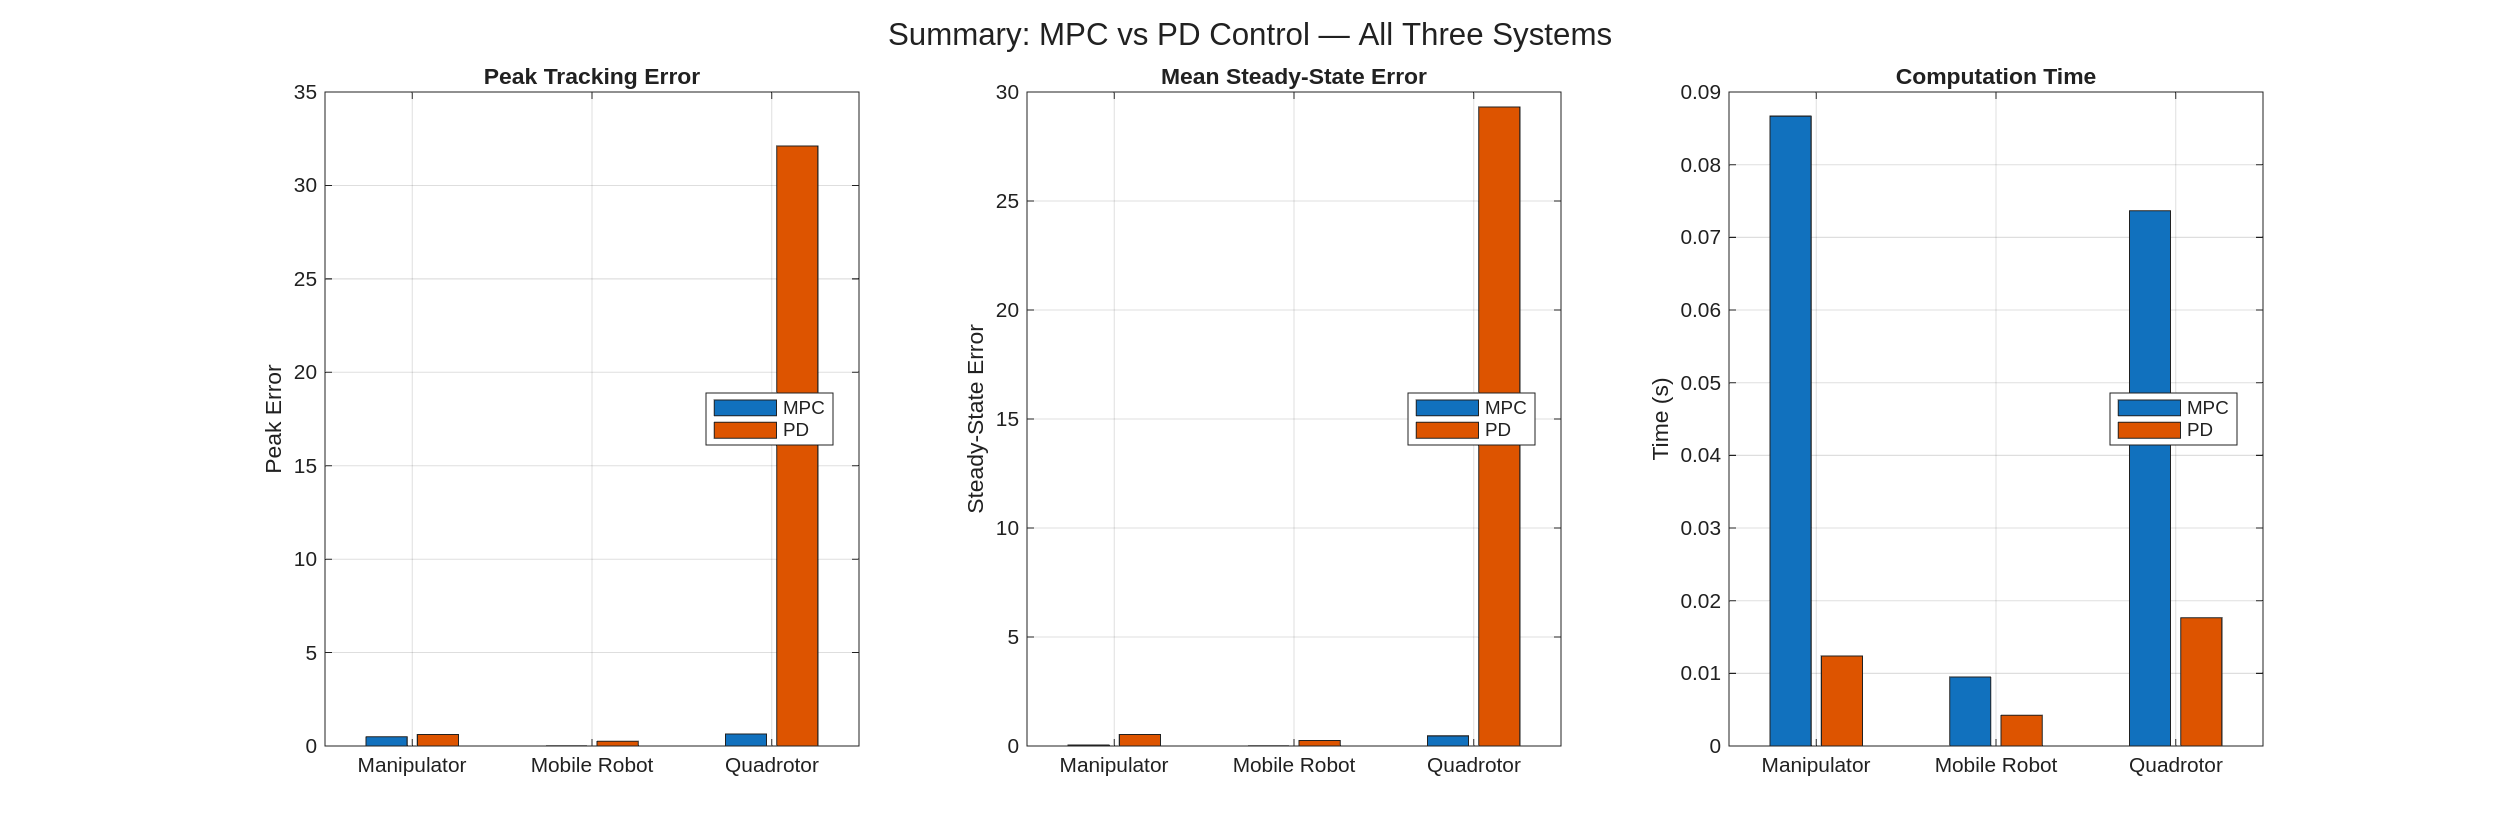
\includegraphics[width=0.92\textwidth,keepaspectratio]{images/week_03/Summary_MPC_vs_PD_for_All_Systems.png}
    \caption{Summary MPC vs PD for all systems.}
\end{figure}

\begin{figure}[ht]
    \centering
    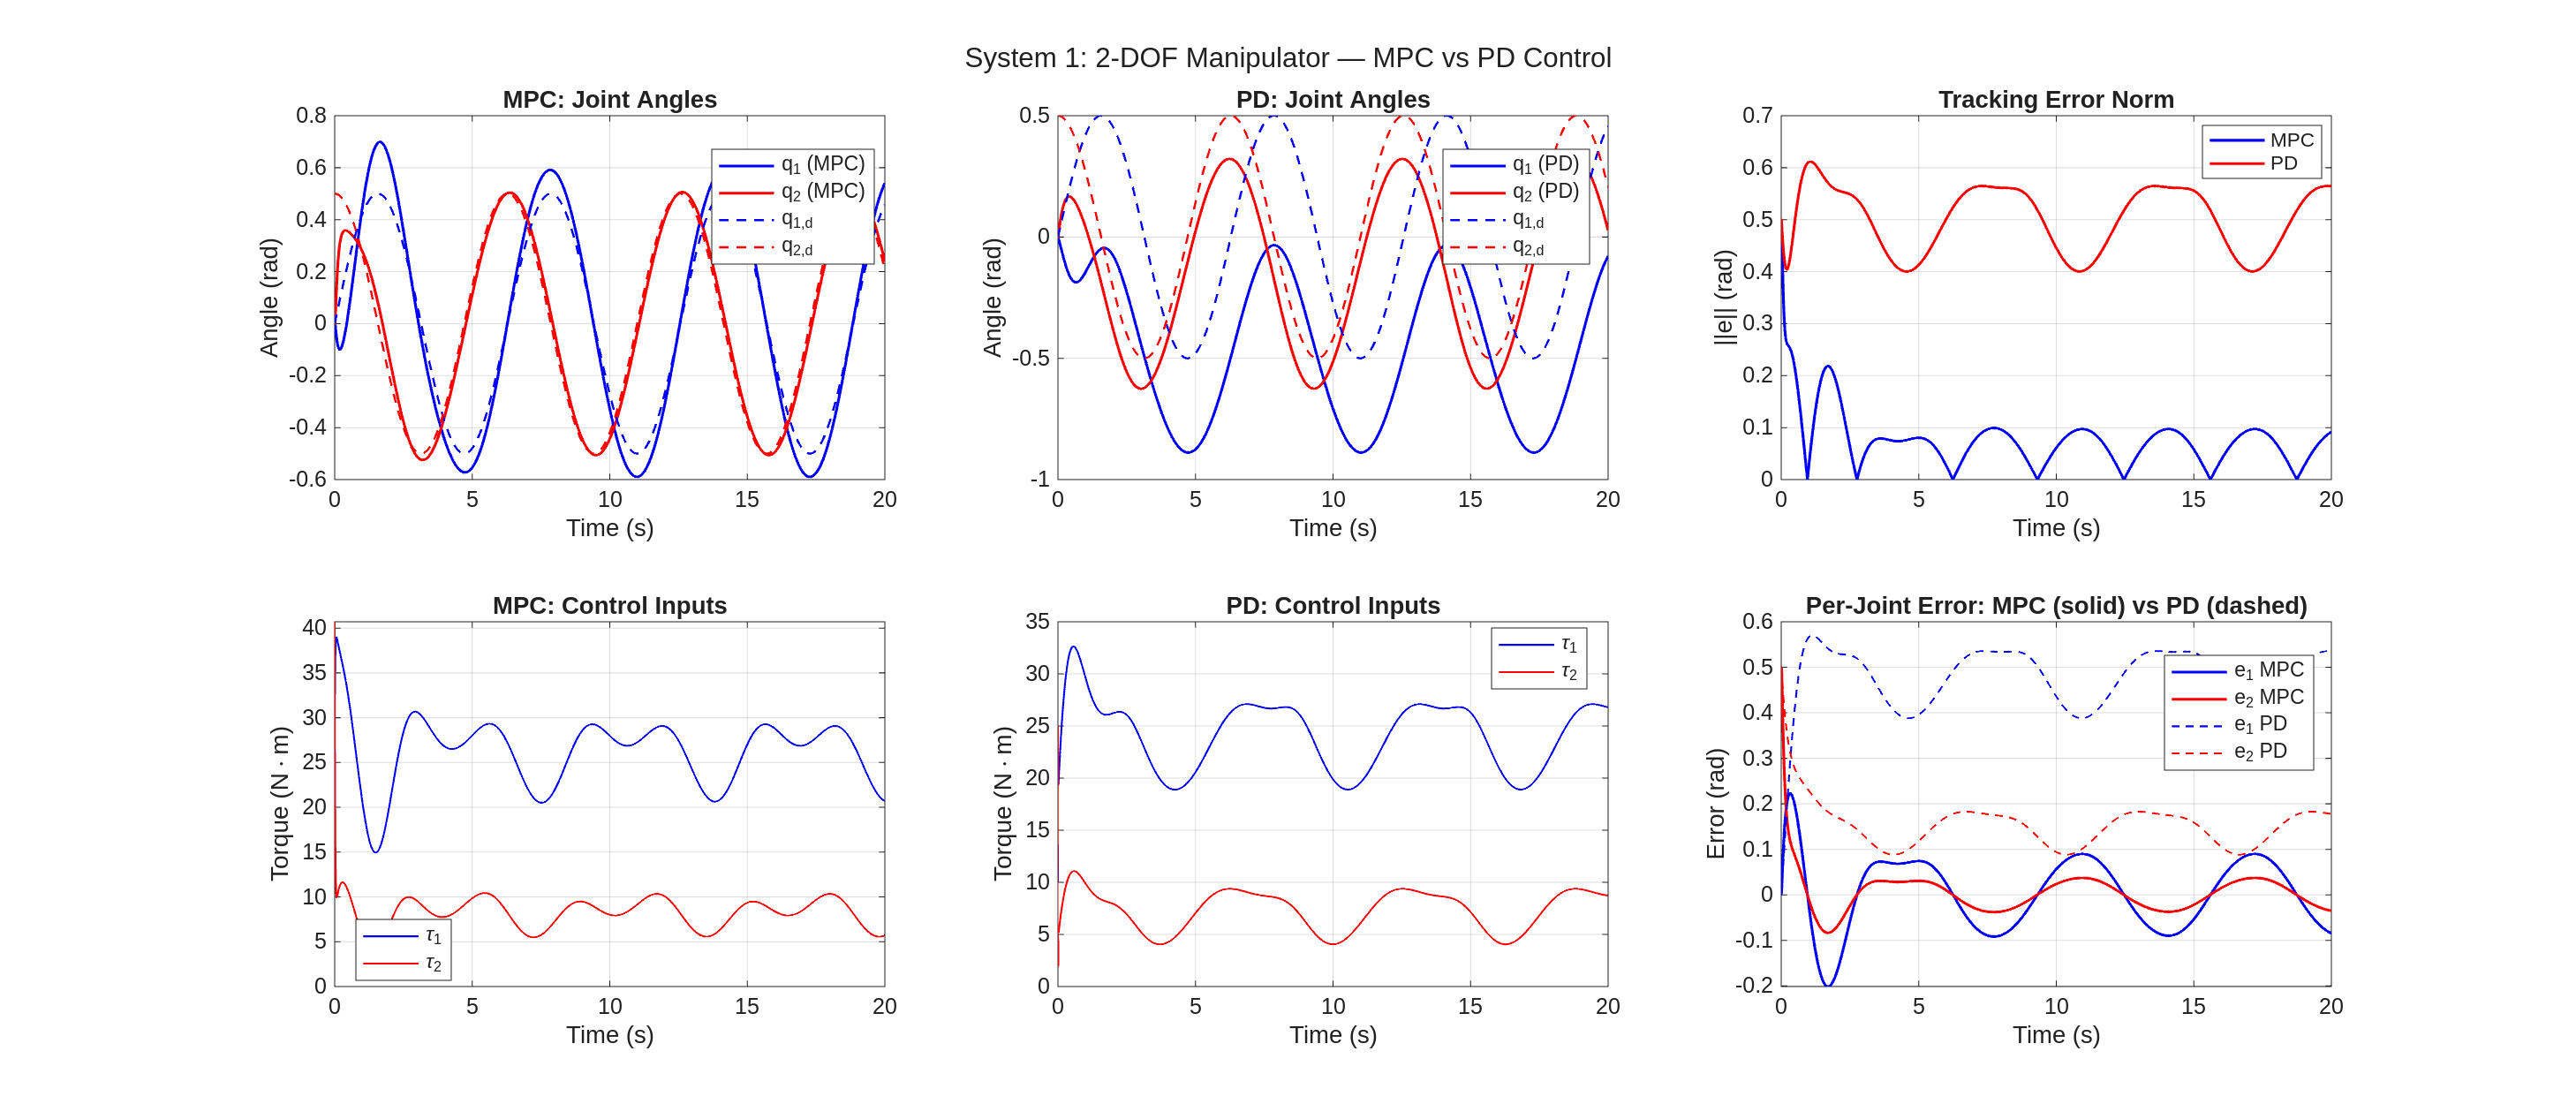
\includegraphics[width=0.92\textwidth,keepaspectratio]{images/week_03/System_1_2-DOF_Manipulator_MPC_vs_PD.png}
    \caption{System 1 2 DOF manipulator MPC vs PD.}
\end{figure}

\begin{figure}[ht]
    \centering
    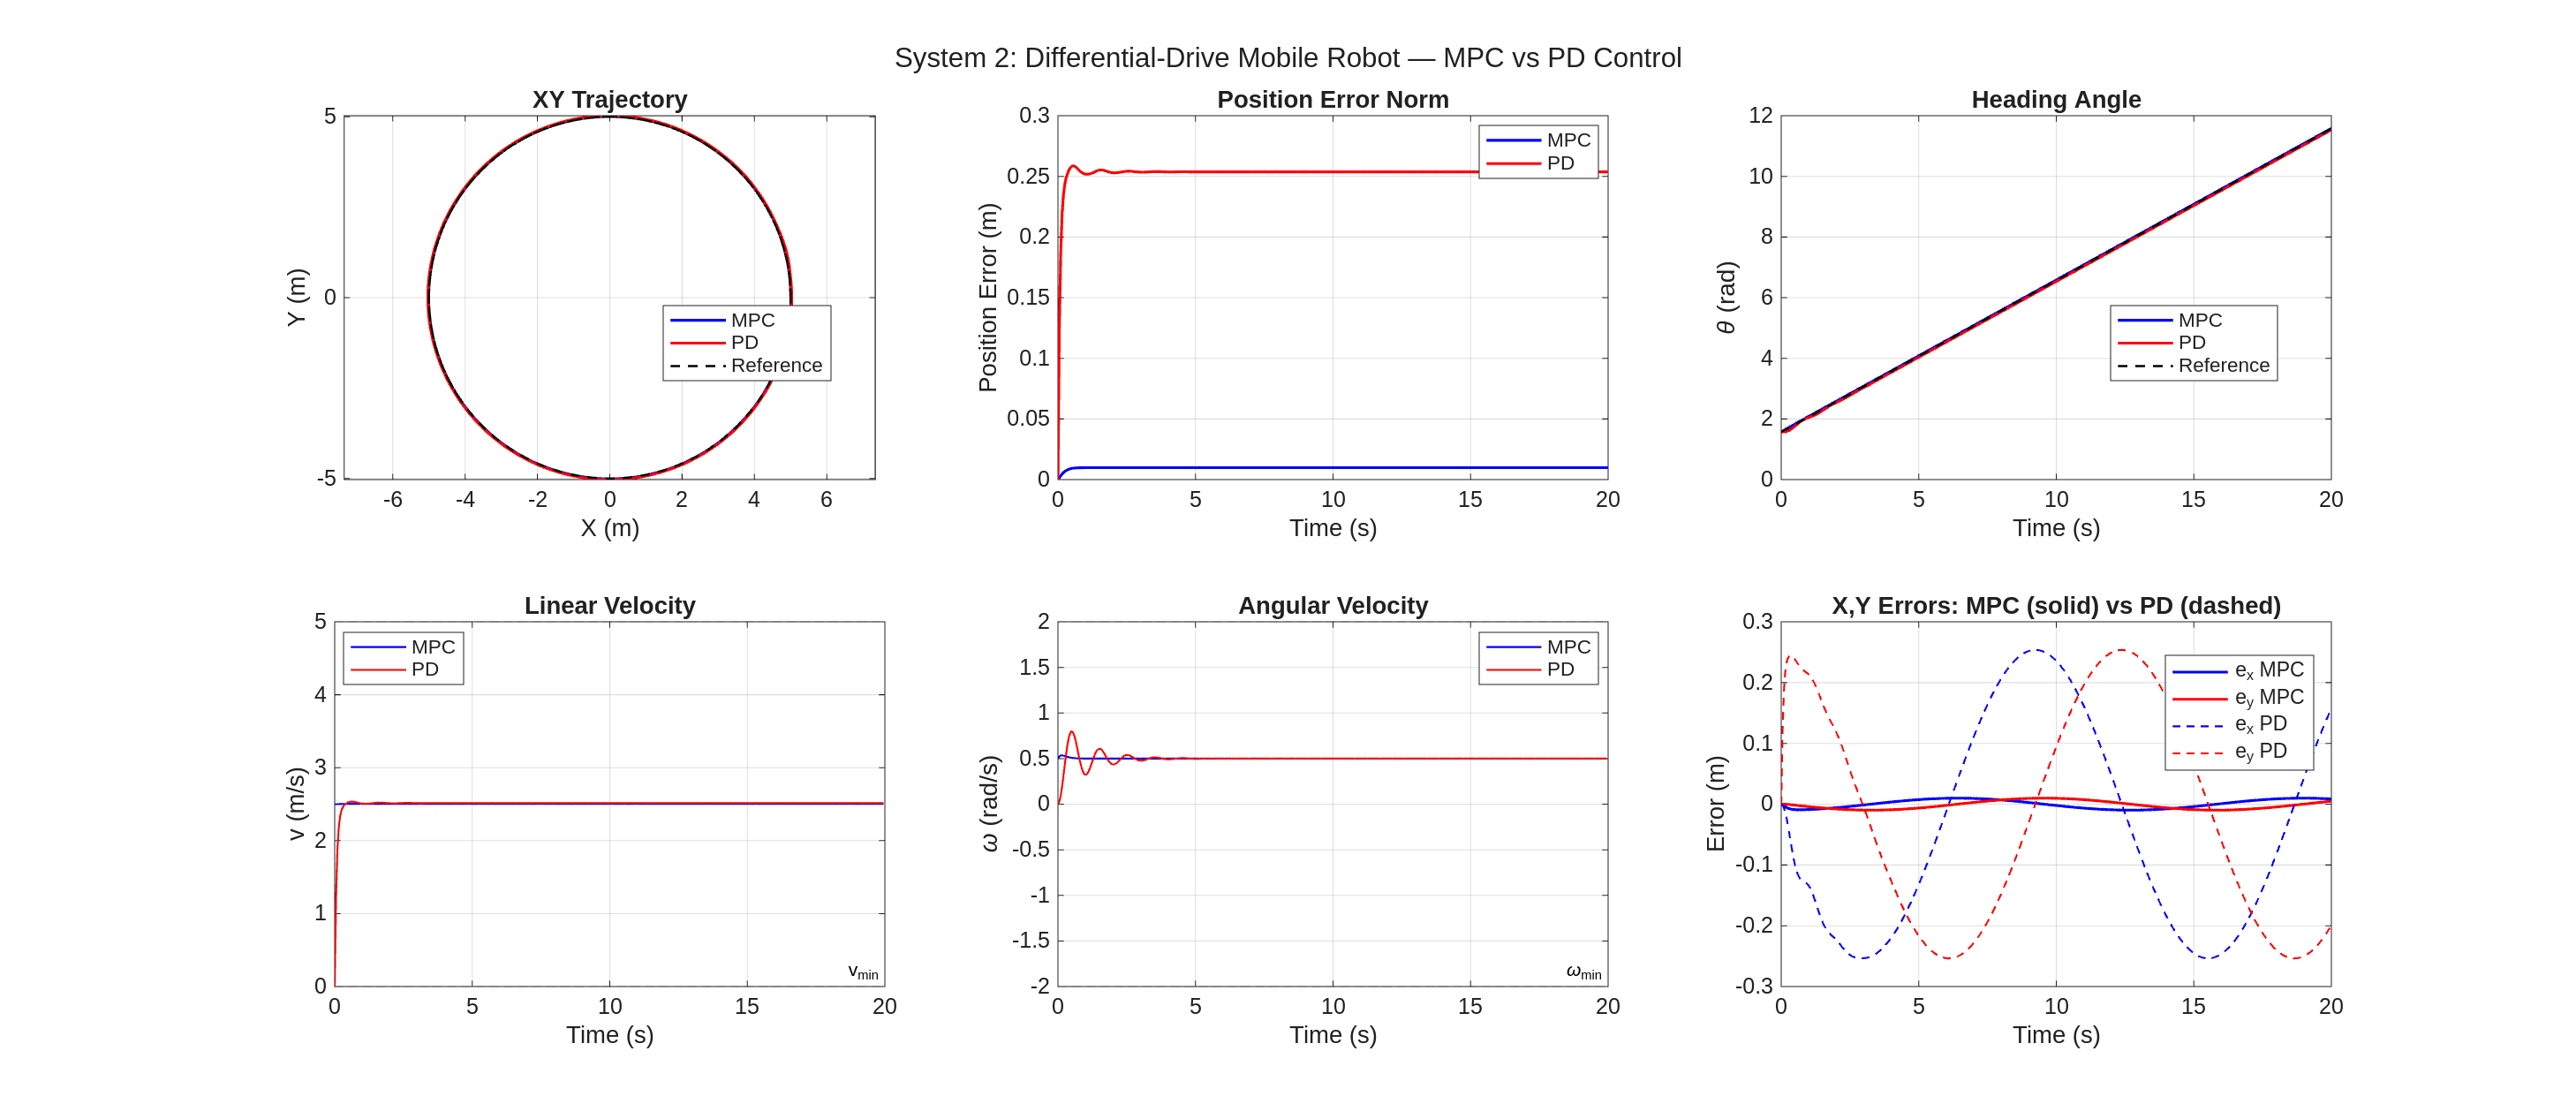
\includegraphics[width=0.92\textwidth,keepaspectratio]{images/week_03/System_2_Mobile_Robot_MPC_vs_PD.png}
    \caption{System 2 mobile robot MPC vs PD.}
\end{figure}

\begin{figure}[ht]
    \centering
    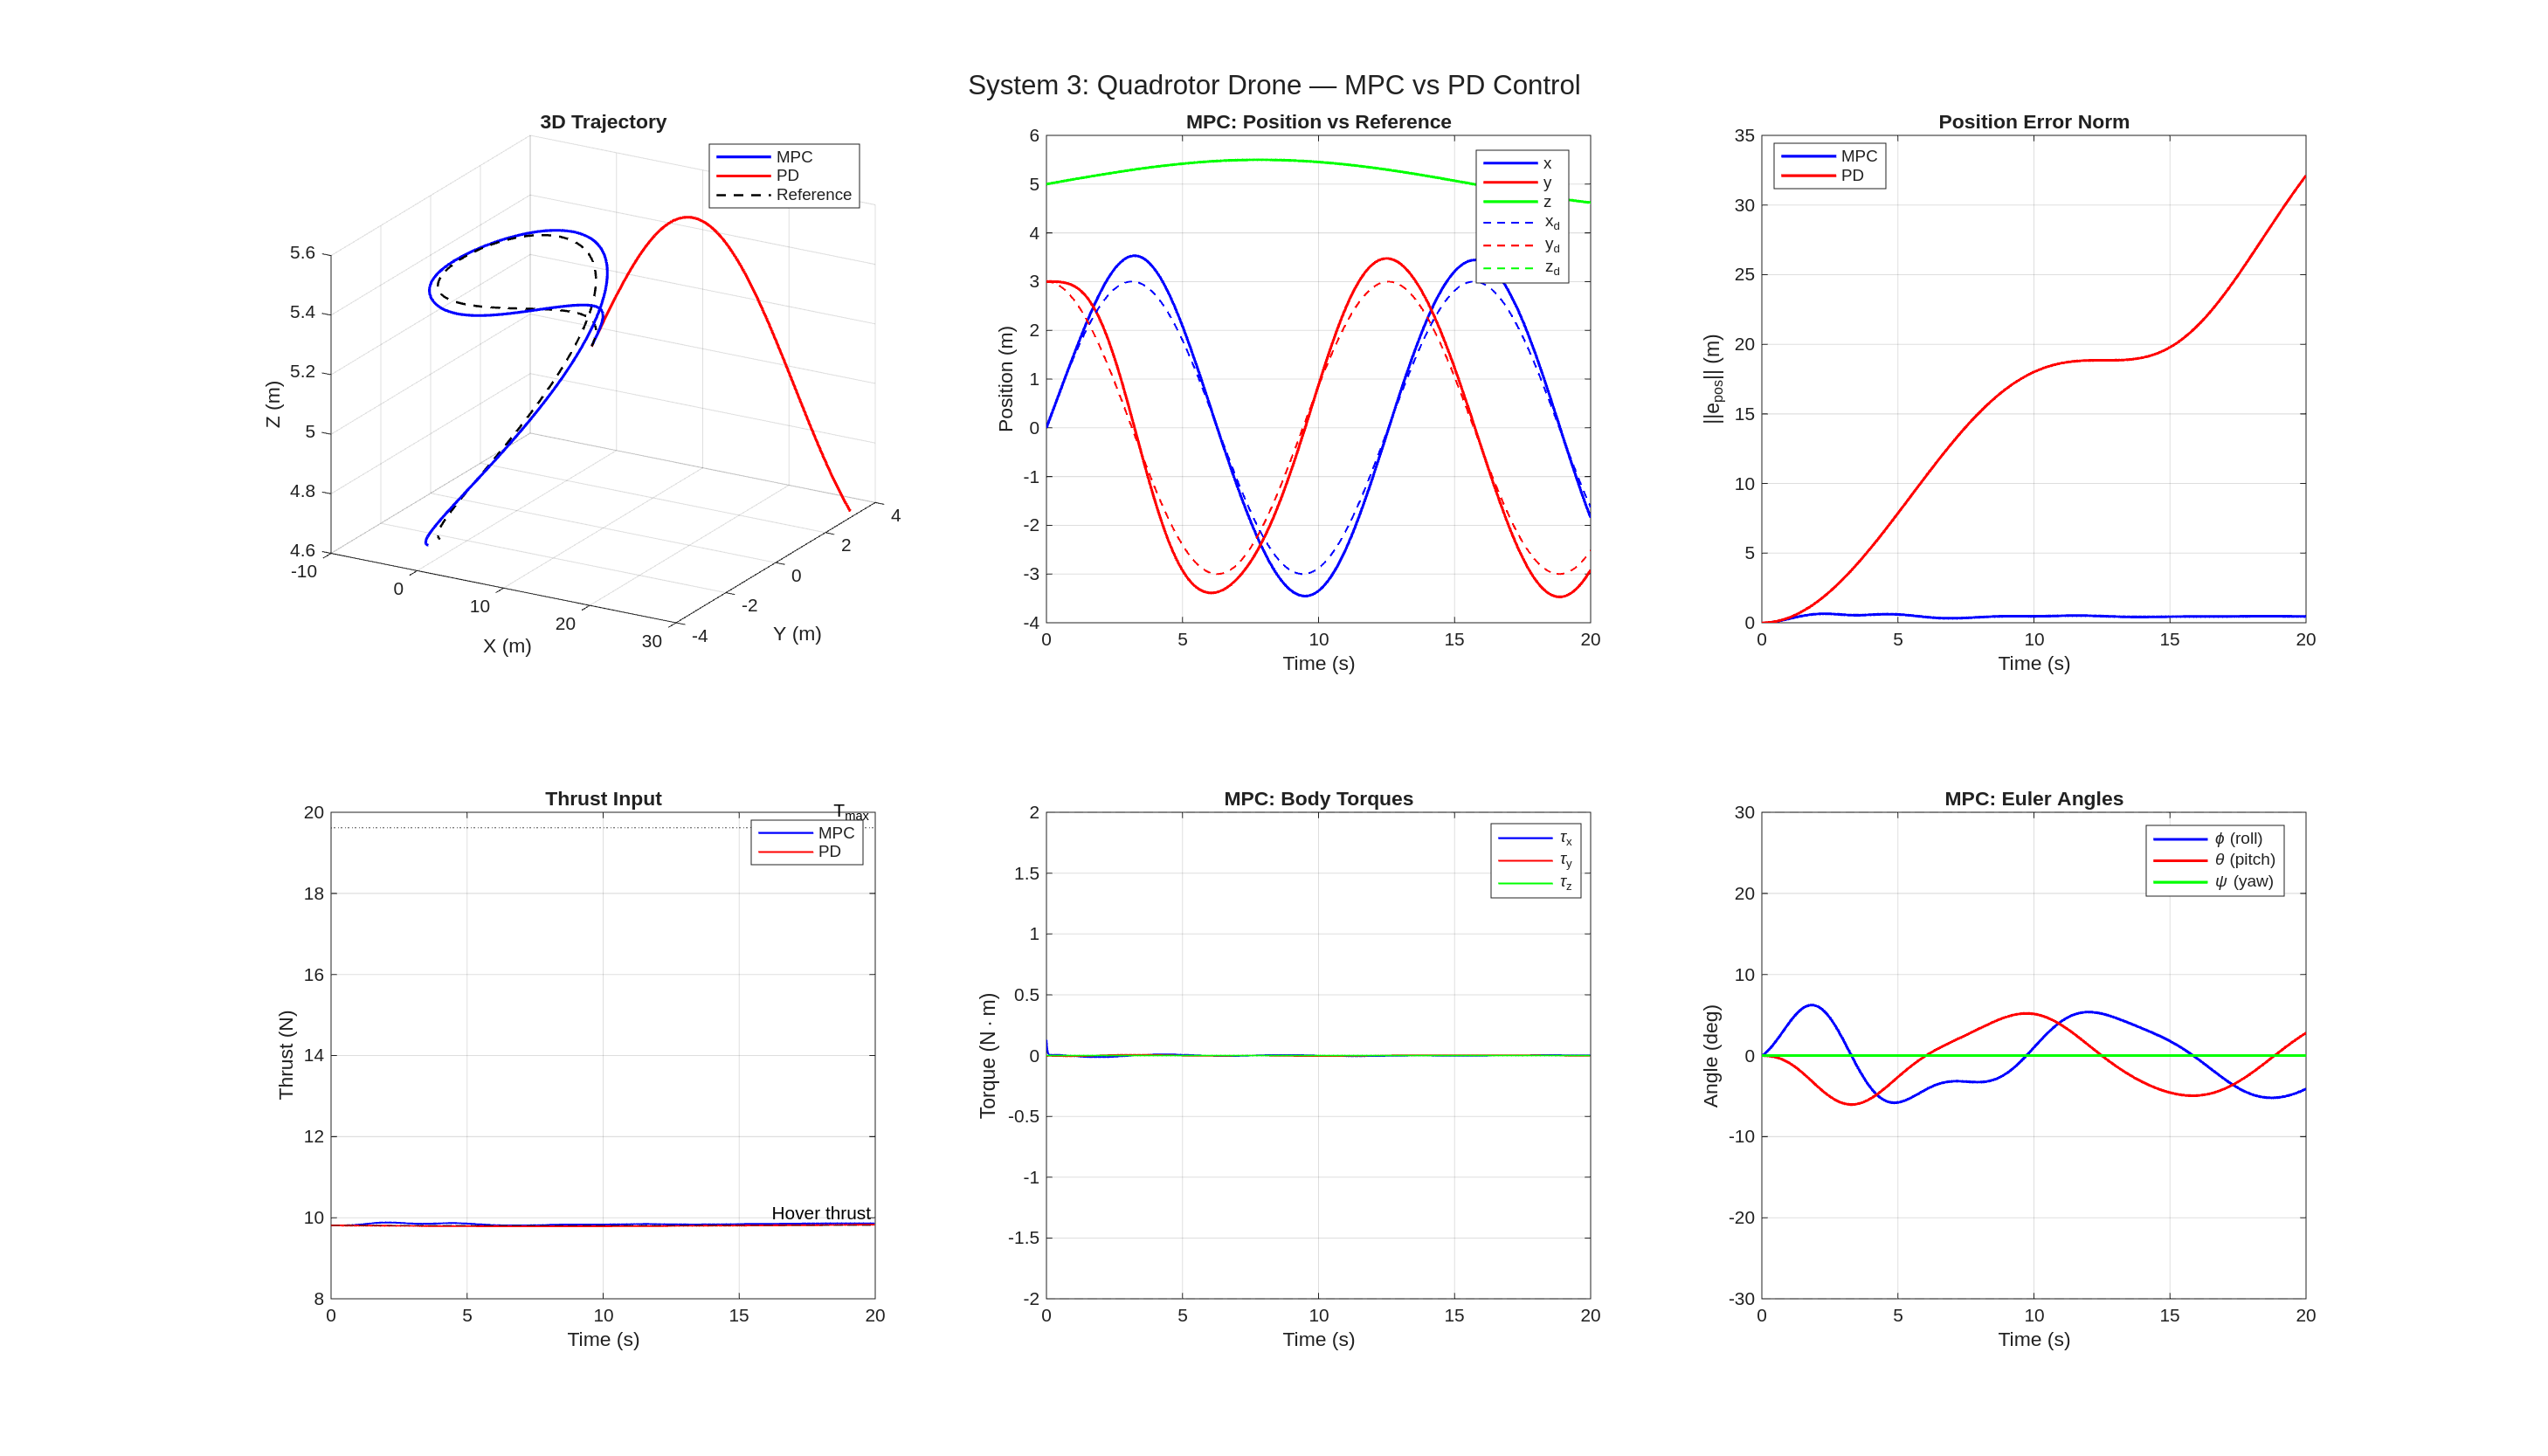
\includegraphics[width=0.92\textwidth,keepaspectratio]{images/week_03/System_3_Quadrotor_MPC_vs_PD.png}
    \caption{System 3 quadrotor MPC vs PD.}
\end{figure}

\section{Summary and Next Steps}

\subsection{Summary \& Key Takeaways}

\subsection{Core MPC Equations}

\begingroup\footnotesize
\begin{longtable}[]{@{}ll@{}}
\toprule\noalign{}
Equation & Description \\
\midrule\noalign{}
\endhead
\bottomrule\noalign{}
\endlastfoot
\(x_{k+1} = A\,x_k + B\,u_k\) & Discrete-time linear system model \\
\(\mathbf{X} = \mathcal{A}\,x_k + \mathcal{B}\,\mathbf{U}\) & Stacked state prediction over horizon \(N\) \\
\(J = (\mathbf{X} - \mathbf{X}_{\text{ref}})^T \mathbf{Q}_N (\mathbf{X} - \mathbf{X}_{\text{ref}}) + \mathbf{U}^T \mathbf{R}_N \mathbf{U}\) & Quadratic cost function \\
\(\mathbf{U}^* = (\mathcal{B}^T \mathbf{Q}_N \mathcal{B} + \mathbf{R}_N)^{-1} \mathcal{B}^T \mathbf{Q}_N (\mathbf{X}_{\text{ref}} - \mathcal{A}\,x_k)\) & Optimal control law (unconstrained) \\
\(u_k = \mathbf{U}^*(1{:}m)\) & Receding horizon: apply only first input \\
\end{longtable}\endgroup

\subsection{MPC vs Computed Torque Control}

\begingroup\footnotesize
\begin{longtable}[]{@{}lll@{}}
\toprule\noalign{}
Property & MPC & Computed Torque \\
\midrule\noalign{}
\endhead
\bottomrule\noalign{}
\endlastfoot
\textbf{Model Knowledge} & Requires linear (or nonlinear) model; can use approximate models with re-linearisation & Requires full nonlinear dynamics \(M(q)\), \(C(q,\dot{q})\), \(G(q)\) \\
\textbf{Constraint Handling} & Systematically incorporates state and control constraints in the optimisation & No built-in constraint handling; requires ad-hoc saturation or anti-windup \\
\textbf{Computation} & Solves a QP at every time step; computational cost grows with \(N\), \(n\), \(m\) & Evaluates \(M\), \(C\), \(G\) and a matrix-vector product; very fast per step \\
\textbf{Tracking Accuracy} & Optimal within the prediction horizon; slightly conservative due to linearisation & Perfect tracking with exact model (nonlinear cancellation) \\
\textbf{Multi-Objective} & Naturally balances tracking, energy, and constraints through cost weights & Single objective: tracking error minimisation \\
\textbf{Robustness} & Feedback through receding horizon; can incorporate robust/stochastic extensions & Sensitive to model mismatch; requires additional robust terms \\
\textbf{Best For} & Systems with constraints, slow-medium dynamics, trajectory optimisation & Fast manipulator control with known dynamics, high-rate servo loops \\
\end{longtable}\endgroup

\subsubsection{Key Takeaway 1}

MPC converts the control problem into a \textbf{repeated optimisation} problem. The quality of the controller depends directly on the quality of the model and the tuning of \(N\), \(Q\), \(R\).

\subsubsection{Key Takeaway 2}

The receding-horizon strategy provides \textbf{implicit feedback}: by re-solving at every step, MPC naturally rejects disturbances and compensates for model errors.

\subsubsection{Key Takeaway 3}

MPC\textquotesingle s greatest strength over computed torque is \textbf{constraint handling}. Real actuators have limits; MPC respects them by design.

\subsubsection{Key Takeaway 4}

Computed torque remains superior when the dynamics are well-known and the control loop must run at \textbf{very high rates} (\textgreater{} 1 kHz) where solving a QP is too expensive.

\subsection{Next Week: Adaptive Control}

\textbf{Building on Weeks 1 and 2, we will cover:}

\begin{itemize}
\tightlist
\item
  Parameter estimation and adaptive control for manipulators with unknown dynamics
\item
  Model Reference Adaptive Control (MRAC)
\item
  Linearity-in-parameters and the adaptive computed torque controller
\item
  Stability proofs for adaptive systems using Lyapunov-based methods
\end{itemize}

\subsection{Preparation}

\begin{itemize}
\tightlist
\item
  Complete all MATLAB activities from today and save your scripts
\item
  Review the linearity-in-parameters property from Week 1 (Section 1.4, Property 3)
\item
  Think about: \emph{"If the controller does not know \(M(q)\), \(C(q,\dot{q})\), or \(G(q)\), how could it learn these online while still maintaining stability?"}
\item
  Read about parameter convergence and persistent excitation
\end{itemize}

\textbf{Control for Robots}

Advanced Robotics Programme \textbar{} Academic Year 2025--26

Week 2: Model Predictive Control (MPC)

This lecture material is for educational use only.
